\documentclass[12pt]{article}

\usepackage{sbc-template}
\usepackage{graphicx,url}
\usepackage[utf8]{inputenc}
\usepackage[brazil]{babel}
\usepackage[latin1]{inputenc}  

     
\sloppy

\title{ENGENHARIA DE SOFTWARE\\ PADRÕES DE PROJETO DE SOFTWARE}

\author{Vinícius Eduardo Alves Oliveira\inst{1}}


\address{Instituto Federal de Educação, Ciência e Tecnologia São Paulo 
  (IFSP)\\
  Campus Votuporanga -- Votuporanga -- SP -- Brazil
  \email{vinicius.oliveira@aluno.ifsp.edu.br}
}

\begin{document} 

\maketitle

\begin{abstract}
  Design patterns are a concept used to explore the uniformity of designs across software applications. They provide a set of established solutions, or blueprints, for solving problems and how to build software. Each pattern describes a particular process or structure that is repeated in the design space, making it easier for engineers and developers to create similar designs.
\end{abstract}
     
\begin{resumo} 
  Os padrões de projeto são um conceito usado para explorar a uniformidade de designs entre aplicações de software. Eles fornecem um conjunto de soluções estabelecidas, ou projeto, para a solução de problemas e como construir software. Cada padrão descreve um determinado processo ou estrutura que se repete uma e outra vez no espaço de projeto, tornando mais fácil para engenheiros e desenvolvedores a criação de projetos similares.
\end{resumo}


\section{Introdução}

Atualmente, durante o fluxo de desenvolvimento de um software, é comum nos 
depararmos com problemas que muitas vezes são recorrentes, ou podem se aproveitar 
de uma mesma técnica de solução. Sendo assim, foram criados os padrões de 
projetos, que oferecem soluções reutilizáveis de software para estes 
problemas recorrentes.

"Uma coisa que os melhores projetistas sabem que não devem fazer é resolver 
cada problema a partir de princípios elementares ou do zero. Em vez disso, 
eles reutilizam soluções que funcionaram no passado. Quando encontram uma 
boa solução, eles a utilizam repetidamente. Consequentemente, você 
encontrará padrões, de classes e de comunicação entre objetos, que 
reaparecem frequentemente em muitos sistemas orientados a objetos. 
Esses padrões resolvem problemas específicos de projetos e tornam os 
projetos orientados a objetos mais flexíveis e, em última instância, 
reutilizáveis. Eles ajudam os projetistas a reutilizar projetos 
bem-sucedidos ao basear os novos projetos na experiência anterior. 
Um projetista que está familiarizado com tais padrões pode aplicá-los 
imediatamente a diferentes problemas de projeto, sem necessidade de 
redescobri-los." \cite{gof}


\section{Padrões de Projeto} \label{sec:firstpage}

Padrões de projeto são soluções já validadas para problemas específicos, 
assim como peças de concreto pré-moldado utilizadas na construção de 
uma casa, os padrões de projeto oferecem soluções padrões para 
problemas já conhecidos no processo de desenvolvimento de software, 
sendo possível personalizá-los para melhor atender o seu cenário.

"... O padrão não é um pedaço de código específico, mas um conceito geral 
para resolver um problema em particular. Você pode seguir os detalhes do 
padrão e implementar uma solução que se adeque às realidades do seu 
próprio programa." \cite{guru}

Segundo \cite{gof}, podemos categorizar os padrões de projeto por sua 
intenção, sendo essas:

\begin{itemize}
\item Padrões de Criação
\item Padrões Comportamentais
\item Padrões Estruturais
\end{itemize}

Durante o desenvolvimento deste artigo, estas categorias serão 
abordadas com mais detalhes, junto a breve resumo dos padrões de 
projetos que as compõem, a Figura ~\ref{fig:fig1} demonstra
quais são estes padrões e suas relações.

\begin{figure}[ht]
\centering
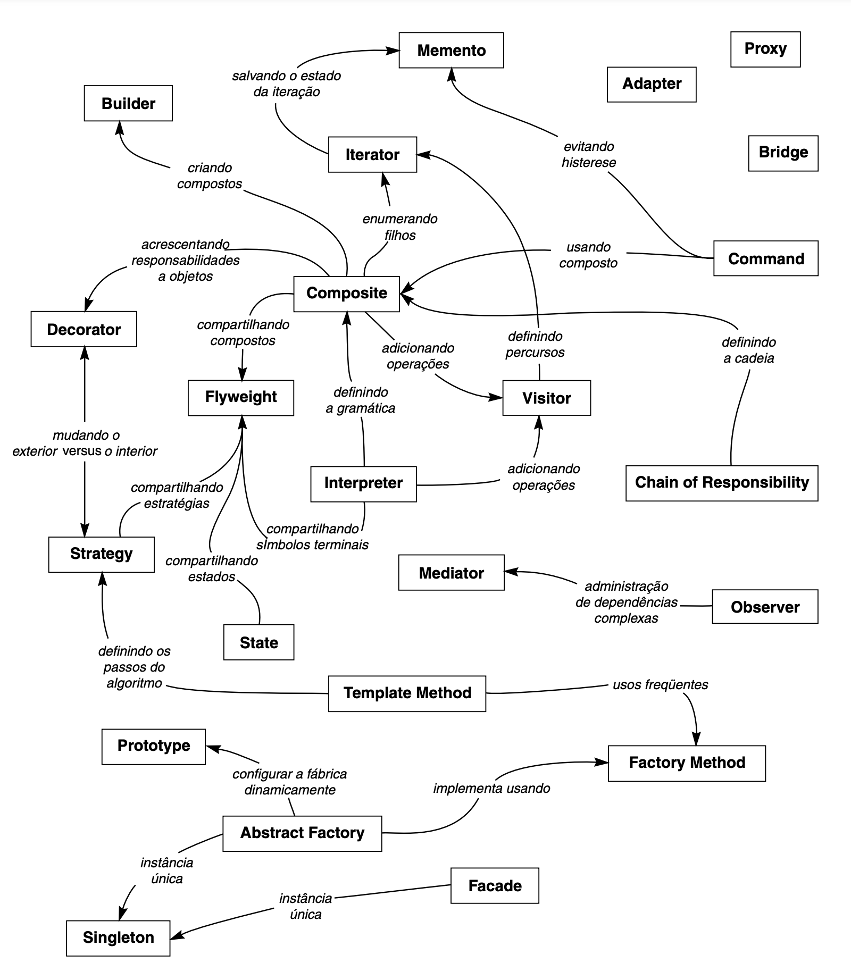
\includegraphics[width=.9\textwidth]{Imagem1.png}
\caption{Relacionamento entre padrões de projeto. \cite{gof}}
\label{fig:fig1}
\end{figure}

\subsection{Padrões de Criação}

Segundo \cite{devmedia_padroes}, os padrões de criação são aqueles 
que abstraem e ou adiam o processo criação dos objetos. Eles ajudam 
a tornar um sistema independentemente de como seus objetos são 
criados, compostos e representados.

Sendo assim, os padrões de criação se tornam crescentemente mais 
importantes, de acordo com a evolução do software, de maneira que 
dependam da composição de objetos, no lugar da herança de classes.  

Utilizar a composição possibilita que objetos sejam criados sem a 
necessidade de expor componentes internos, permitindo que o 
comportamento de sua criação seja definido dinamicamente, 
alterando o paradigma de codificar um comportamento rígido, para 
um conjunto de menores comportamentos, podendo estes, serem 
reunidos para criação de comportamentos complexos.

De acordo com \cite{gof} e \cite{guru}, os principais 
padrões de projeto de criação são:

\begin{itemize}
\item \textit{Factory Method}: fornece uma interface para criar 
objetos em uma superclasse, mas permite que as subclasses alterem 
o tipo de objetos que serão criados.
\item \textit{Abstract Factory}: permite a produção de famílias 
de objetos relacionados sem ter que especificar suas classes 
concretas.
\item \textit{Builder}: permite a construção de objetos complexos 
passo a passo, possibilitando a produção de diferentes tipos e 
representações de um objeto usando o mesmo código de construção.
\item \textit{Prototype}: permite copiar objetos existentes sem 
tornar o código dependente de suas classes.
\item \textit{Singleton}: garante que uma classe tenha apenas 
uma instância, enquanto provê um ponto de acesso global para 
essa instância.
\end{itemize}

\subsection{Padrões Estruturais}

Segundo \cite{gof}, os padrões estruturais se preocupam com a forma 
como classes e objetos são compostos para formar estruturas maiores. 
Os padrões estruturais de classes utilizam a herança para compor 
interfaces ou implementações. Dando um exemplo simples, considere 
como a herança múltipla mistura duas ou mais classes em uma outra. 
O resultado é uma classe que combina as propriedades das suas 
classes ancestrais. Esse padrão é particularmente útil para fazer 
bibliotecas de classes desenvolvidas independentemente 
trabalharem juntas.

Sendo assim, padrões estruturais focam em como construir suas 
classes e objetos, de modo que consigam se complementar e 
estender suas funcionalidades, enquanto gera código 
reutilizável e sem duplicação.

De acordo com \cite{gof} e \cite{guru}, os principais padrões 
de projeto estruturais são:

\begin{itemize}
\item \textit{Adapter}: permite a colaboração de objetos de interfaces 
incompatíveis.
\item \textit{Bridge}: permite que uma classe grande ou um conjunto 
de classes intimamente ligadas sejam divididas em abstração e 
implementação, que podem ser desenvolvidas independentemente 
umas das outras.
\item \textit{Composite}: permite a composição de objetos 
em estruturas de árvores, habilitando trabalhar com estas 
estruturas de forma parecida a objetos individuais.
\item \textit{Decorator}: permite o acoplamento de novos comportamentos 
a objetos, os encapsulando dentro de objetos que contém 
os comportamentos.
\item \textit{Facade}: fornece uma interface simplificada para 
uma biblioteca, um framework, ou qualquer conjunto 
complexo de classes.
\item \textit{Flyweight}: permite reduzir o consumo de RAM ao 
compartilhar partes comuns de estado entre os múltiplos 
objetos ao invés de manter todos os dados em cada objeto.
\item \textit{Proxy}: permite a criação de um substituto ou um espaço 
reservado para outro objeto. Um proxy controla o acesso ao objeto 
original, permitindo que você faça algo ou antes ou depois do 
pedido chegar ao objeto original.
\end{itemize}

\subsection{Padrões Comportamentais}

Segundo \cite{gof} os padrões comportamentais se preocupam com 
algoritmos e a atribuição de responsabilidades entre objetos. 
Os padrões comportamentais não descrevem apenas padrões de objetos 
ou classes, mas também os padrões de comunicação entre eles. 
Esses padrões caracterizam fluxos de controle difíceis de seguir 
em tempo de execução. Eles afastam o foco do fluxo de controle 
para permitir que você se concentre somente na maneira como os 
objetos são interconectados.

Sendo assim, padrões comportamentais focam em como estruturar o 
fluxo de seu software, trazendo maneiras de como suas classes e 
objetos podem se comunicar, transferindo dados através deles, 
além de formas para organizar suas regras de negócio, evitando 
alto acoplamento e duplicação de código.

De acordo com \cite{gof} e \cite{guru}, os principais padrões 
de projeto estruturais são:

\begin{itemize}
\item \textit{Chain of Responsibility}: permite que pedidos sejam 
transferidos dentro de uma corrente de handlers.
\item \textit{Command}: transforma um pedido em um objeto 
independente que contém toda a informação sobre o mesmo. 
Essa transformação permite que você parametrize métodos com 
diferentes pedidos, atrase ou coloque a execução do pedido 
em uma fila, e suporte operações que não podem ser feitas.
\item \textit{Iterator}: permite percorrer elementos de uma 
coleção sem expor as representações dele (lista, pilha, árvore, etc.).
\item \textit{Mediator}: reduz a interdependência entre 
objetos, forçando que a comunicação entre eles ocorra 
através de um intermediador.
\item \textit{Memento}: permite que o estado de um objeto 
seja salvo e restaurando, sem revelar os detalhes de 
sua implementação.
\item \textit{Observer}: permite a definição de um mecanismo 
de assinatura para notificar múltiplos objetos sobre quaisquer 
eventos que aconteçam com o objeto que eles estão observando.
\item \textit{State}: permite que um objeto altere seu 
comportamento quando seu estado interno muda.
\item \textit{Strategy}: permite a definição de uma família 
de regras de negócio, em classes separadas, porém com seus 
objetos intercambiáveis.
\item \textit{Template Method}: define o esqueleto de um 
algoritmo na superclasse, mas deixa as subclasses sobrescreverem 
etapas específicas do algoritmo sem modificar sua estrutura.
\item \textit{Visitor}: permite que as regras de negócio sejam 
separadas dos objetos que as utilizam.
\end{itemize}

\section{Conclusão}

Utilizando padrões de projeto, conseguimos criar softwares cada 
vez mais flexíveis, escaláveis e reutilizáveis, com soluções já 
provadas para problemas recorrentes no fluxo de desenvolvimento 
de software. Por se tratar de padrões criados com linguagem clara 
e concisa, utilizando um alto nível de abstração, facilitam 
também a passagem de conhecimento dentre arquitetos de software.

Dessa forma, concluo que os padrões de projeto auxiliam imensamente 
no desenvolvimento de software, se tornando quase indispensáveis 
durante a construção de softwares modernos, reduzindo a carga 
cognitiva utilizada pelos integrantes do time de desenvolvimento 
e trazendo agilidade na resolução de problemas arquiteturais e 
operacionais do software.



\section{Referências}

\bibliographystyle{sbc}
\bibliography{sbc-template}

\end{document}
